%!TEX root = ../../thesis.tex

It is clear from (\ref{eq:event_rate}) that the luminosity delivered to the detector is a 
key input when studying \pp collisions at the \ac{LHC}. It is directly proportional to the 
expected number of events, and uncertainties in its value will be propagated to measured 
cross sections. The measurement of the luminosity delivered to the ATLAS detector is 
described in \Section~\ref{sec:dataset:lumi}, followed by a description of the dataset 
used in this thesis.



\subsection{Luminosity measurement}
\label{sec:dataset:lumi}

At the \ac{LHC}, the number of inelastic \pp interactions per bunch crossing follows a 
Poisson distribution, with a mean value $\mu$. As mentioned in \Section~\ref{sec:lhc}, 
a large luminosity results in $\mu > 1$ (a condition known as pile-up). Thus, the 
luminosity $L$ can be inferred ``online'' from a measurement of $\mu$, using
\begin{equation}
	L = \frac{\mu n_b f_{\text{rev}}}{\sigma_{\text{inel}}}
	= \frac{\mu_{\text{vis}} n_b f_{\text{rev}}}{\sigma_{\text{vis}}}
	\label{eq:lumi_measure}
\end{equation}
where $n_b$ is the number of bunches per beam, $f_{\text{rev}}$ is the \ac{LHC} revolution 
frequency, and $\sigma_{\text{inel}}$ is the inelastic \pp cross section. The 
expression is rewritten in terms of ``visible'' quantities, owing to inefficiencies in the
detector and algorithm used to measure $\mu$.

The \ac{BCM} and LUCID detectors, respectively situated \unit{2}{\metre} and 
\unit{17}{\metre} down the beamline from the interaction point, each provide 
bunch-by-bunch luminosity measurements. The \ac{BCM} consists of sixteen small diamond 
sensors, and was primarily designed to issue beam-abort requests when beam losses risk 
damaging the ATLAS detector. Diamond was chosen instead of silicon due to its 
radiation-hardness and short time resolution (\unit{\about0.7}{\nano\second}).
LUCID consists of sixteen aluminium tubes of C$_4$F$_{10}$ gas, which radiate and collect 
Cherenkov photons when struck by charged particles.

\ac{BCM} and LUCID are calibrated during dedicated van der Meer (vdM) scans, effectively 
determining $\sigma_{\text{vis}}$ in (\ref{eq:lumi_measure}). In a vdM scan, event rates
are measured while the beams are separated in steps of known distance, allowing direct 
measurement of $\varSigma_x$ and $\varSigma_y$. The absolute luminosity is then determined 
through (\ref{eq:lumi_beam}). The uncertainty in the vdM calibration dominates the 
uncertainty in the delivered luminosity \cite{Lumi2011}.



\subsection{Run I dataset}
\label{sec:dataset:dataset}

Data-taking during run I of the LHC was incredibly successful. Some key beam parameters are
displayed in \Table~\ref{tab:dataset} and the pile-up conditions are shown in 
\Figure~\ref{fig:pileup}.

\begin{table}[h]
	\begin{tabular}{lc@{\hskip 0.25in}c@{\hskip 0.25in}c}
	& 2010 & 2011 & 2012 \\
	\hline
	Centre-of-mass energy (\TeV)         & 7 & 7 & 8 \\
	Minimum bunch spacing (\nano\second) & 150 & 50 & 50 \\
	Peak luminosity (\unit{$10^{33}$}{\lumiunits}) & 0.2 & 3.6 & 7.7 \\
	Delivered luminosity (\invfb)       & 0.047 & 5.46 & 22.8 \\
	Recorded luminosity (\invfb)        & 0.044 & 5.08 & 21.3 \\
	Analysed luminosity (\invfb)        & 0     & 5 & 21 \\
	Luminosity uncertainty $\delta L/L$ & 3.5\% & 1.8\% & 2.8\% \\
	\end{tabular}
	\caption{Summary of \pp collision data during run I of the \ac{LHC}. The integrated luminosity analysed in the \HWW search is also shown.}
	\label{tab:dataset}
\end{table}

\begin{figure}[h]
	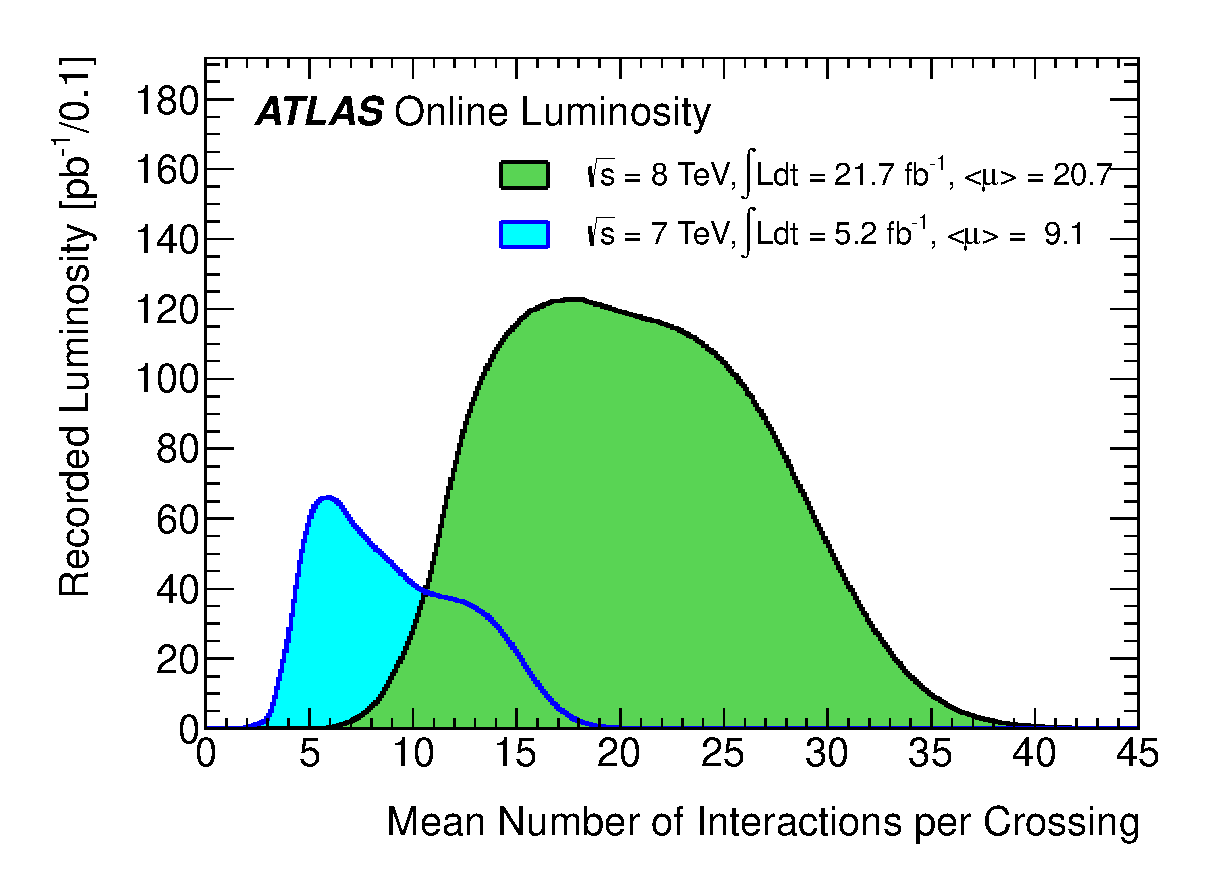
\includegraphics[width=\mediumfigwidth]{tex/experiment/pileup}
	\caption{The mean number of interactions per bunch crossing, $\mu$, for the 2011 (blue)
	and 2012 (green) datasets. These were calculated with an inelastic \pp cross 
	section of \unit{71.5}{\milli\barn} at \unit{$\sqrt{s} = 7$}{\TeV} and 
	\unit{73.0}{\milli\barn} at \unit{$\sqrt{s} = 8$}{\TeV}.}
	\label{fig:pileup}
\end{figure}

